\chapter{Software and Tools}
\label{existing_tech}

The existing system is based on works from previous student projects and master theses. An overview of the present methods and tools will be needed to address some of the current objectives. The following sections will introduce tools and functionality that plays a key role in this project.

\section{Qt}

Qt is a cross-platform software development framework used for developing an application to various software and hardware platforms \cite{qt}. The framework is primarily used with regards to graphical applications as it has a wide range and support of tools for data presentation and interaction. Qt also provides GUI that emulate a native-looking interface. Application and libraries using Qt can be compiled by standard C++ compilers such as Clang, GCC and MinGW. 

The Qt Company provide extensive support and documentation of the framework such that it is easy to get started despite having little knowledge of the framework beforehand. In addition, there are plenty of accessible discussion forums for help and support, and exchanging information among developers.


\section{GeoMod}

The GeoMod software was developed as an environment for simulation and testing of AUVs and tools to handle real life assignments. The software was first developed by Professor Sven Fjeldaas at NTNU for this purpose. The development of the software has since been a collaboration project by several students over the years. From the initial development until this day, substantial changes have been done, e.g. porting between platforms and update of code to keep up with the latest Qt version.


\subsection{Model}
\label{chap:model}

\begin{figure}[ht]
    \centering
    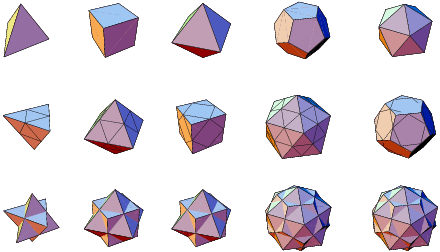
\includegraphics[height=5cm]{images/poly.png}
    \caption[Various type of polyhedrons \cite{polyhedrons}]{Various type of polyhedrons \cite{polyhedrons}.}
    \label{fig:polyhedrons}
\end{figure}

\noindent Vehicles and tools are in GeoMod represented as mathematical geometric models rendered as multiple composed polyhedrons. \Cref{fig:polyhedrons} illustrates how polyhedrons can form various types of shapes to create complex objects. GeoMod manages this by creating nodes with connected edges forming flat regions through the classes \textit{GeomNode} and \textit{GeomEdge}. The acquisition of the project included a few simple models, in addition to a model of a manipulator made from model parts that are linked together. These models, seen from \Cref{fig:viewport}, are used as a basis for the implementation of the control system. They consist, in the current state, of individual source files that are manually hard-coded in the software. 

\begin{figure}[ht]
    \centering
    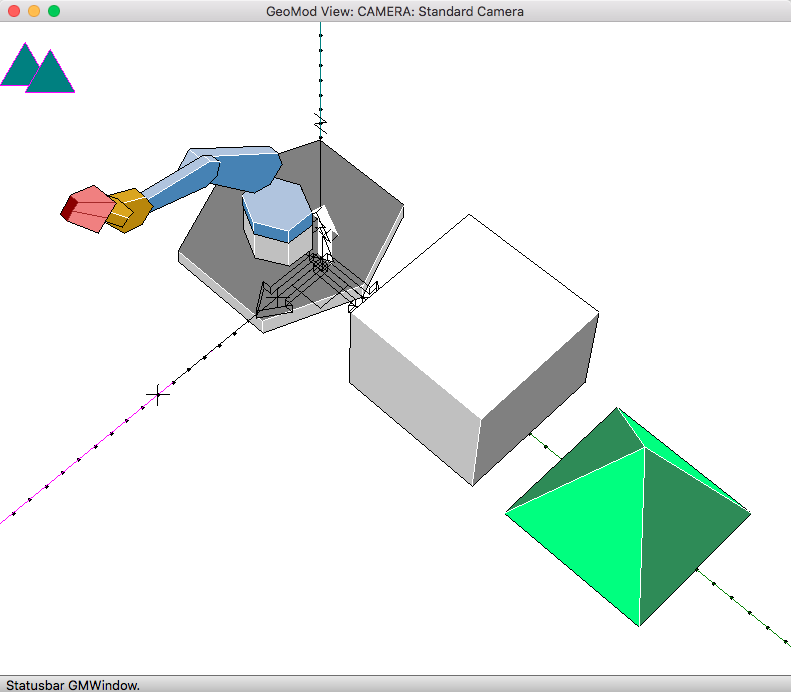
\includegraphics[height=8cm]{images/Models.png}
    \caption[The GeoMod viewport is showing a geometric model of a typical serial manipulator, pyramid and cube]{The GeoMod viewport is showing a geometric model of a typical serial manipulator, pyramid and cube.}
    \label{fig:viewport}
\end{figure}

During this project, there have been other students working in parallel with the development of the software. One of their assignments has been focused on using dynamic linking with the concern of this topic. In the current code, models are statically linked as the program is compiled. The program has to be recompiled if there are changes and updates in the code or library. With dynamic linking, new models can be added during runtime that corresponds to how an autonomous system should respond. This has to be taken into consideration when an implementation of a control system is based on how the models are being handled in the software.


\subsection{Model transformation}

\begin{figure}[ht]
    \centering
    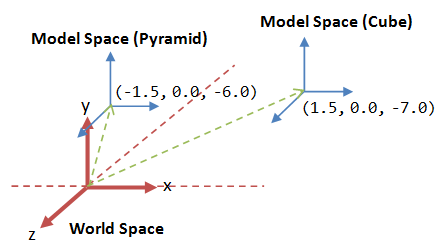
\includegraphics[height=5cm]{images/ModelSpace.png}
    \caption[Model transformation \cite{modelspace}]{Model transformation \cite{modelspace}.}
    \label{fig:modelspace}
\end{figure}

Models in GeoMod consist each of a transformation group of the class \textit{TGroup}, which contains geometric information of the model in Cartesian coordinate system. The class further consists of a basis that allows models to have their own coordinate system (model space). By setting an offset and orientation vector of the basis relative to the main coordinate system (world space), enables models to be moved and rotated in a three dimensional space (\Cref{fig:modelspace}). For the serial manipulator model, the same principle works on the joints. The model parts use an offset vector between the joint basis and the world space for position and orientation to create a linked model. Valid joint movements can be calculated from their bases through subroutines.

The models used in this project came with each a panel for movement when the software was handed over. These panels are very limited as it only has translation and rotation options along one of the three axes. In \Cref{fig:controlcube} shows the panel for the model named "cube" consisting of buttons in the X, Y and Z directions with respect to translation and rotation. Movement is done incrementally as the step value is determined beforehand and hard-coded. 

A panel for movement was included with each model used in this project, when the software was handed over. These panels are very limited considering that there are only translation and rotation options along one of the three axes. In \Cref{fig:controlcube} a panel for the model \textit{Cube} is shown. It consists of buttons for X, Y and Z directions with respect to translation and rotation. Movement is done incrementally as the step value is determined beforehand and hard-coded. The panel also contains a functionality to save the sequence of motion of the model to repeat the same movement. Dejectedly, this feature has not yet been implemented in the currently given version of GeoMod. 

\begin{figure}[ht]
    \centering
    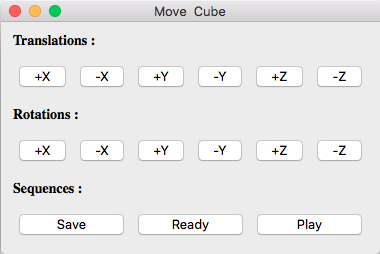
\includegraphics[height=5cm]{images/control_cube.png}
    \caption[Control panel for the cube model]{Control panel for the cube model.}
    \label{fig:controlcube}
\end{figure}


\subsection{Paths}

In GeoMod a basic proof of concept for paths created as a network, have been implemented by Martin Lygre Furevik in his master thesis, Spring 2016. In his work, paths are implemented like models. As models are created with GeomNode and GeomEdge, paths are also formed by edges connected to nodes. Paths and models share many of the same properties and features that can be used interchangeably. This implies that paths can be moved and rotated like models as they also contain geometric data within a transformation group. A network of paths is made of a list of edges and nodes that count as linear or curved lines for guidance. 

The handed GeoMod version included a path object resemblance to a cube. As with dynamic linking, there is also another student working in parallel with this assignment to manage creation and editing of paths at runtime.